\textbf{Paso 1: Estructuración según el patrón MVC}  
Se decidió implementar el patrón Modelo-Vista-Controlador (MVC) para organizar el código y mantener una separación clara de responsabilidades.  
Se crearon tres carpetas principales dentro del proyecto: 

\begin{figure}[H]
    \centering
    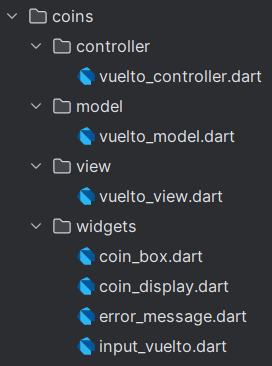
\includegraphics[width=0.4 \textwidth, height=6cm, keepaspectratio]{ej13/cap1.png}
    \caption{Patrón MVC en years}
    \label{fig:ej13il1}
\end{figure}

\textbf{Paso 2: Creación de archivos .dart para cada componente}  
Dentro de cada carpeta se añadieron los archivos correspondientes:  
\begin{itemize}
    \item aniosmodel.dart en model
    \item anioscontroller.dart en controller
    \item aniosview.dart en view
\end{itemize}

\textbf{Paso 3: Desarrollo de los componentes (modelo $\rightarrow$ controlador $\rightarrow$ vista)}  

\textbf{aniosmodel.dart:}  
En este archivo, se programó la lógica para verificar y validar si un año es bisiesto. Se programó la función \texttt{esBisiesto}, que toma un número entero como el año y te devuelve un booleano \texttt{true} o \texttt{false} dependiendo de si cumple con las reglas del calendario para años bisiestos.

Las diferentes reglas son: si un año no se divide por 4, no es bisiesto, si se divide por 4 pero no por 100, entonces sí lo es, y si se divide por 400, también cuenta como bisiesto.

De esta forma, toda esa lógica queda bien guardada en el modelo, apartada de la interfaz y del controlador.

\textbf{anioscontroller.dart:}  
La clase \texttt{AnioController} es la que se pone a manejar lo que el usuario escribe: lo recibe, le hace todas las validaciones necesarias y manda un mensaje claro según lo que encontró.

El método \texttt{procesar} es donde ocurre lo más importante: primero revisa que el campo no esté vacío, luego confirma que sea un número positivo válido y que no supere el límite máximo que tenemos definido (\texttt{maxAnio}). Si todo está bien, consulta al \texttt{AnioModel} usando su método \texttt{esBisiesto} para determinar si el año es bisiesto o no, y por último devuelve un mensaje claro al usuario con el resultado o, si hubo problemas, con el error correspondiente.

De esta forma, el controlador concentra toda la validación y el procesamiento, preservando la división entre los datos en el modelo y la presentación en la vista, y garantizando que la interfaz solo reciba información ya lista y procesada para mostrar.

\textbf{aniosview.dart:}  
En este archivo se diseñó la interfaz de usuario de la aplicación, reuniendo los Widgets necesarios para que el usuario pueda ingresar un año y verificar si es bisiesto de manera sencilla.

Se organizaron los componentes siguiendo una estructura reutilizable:

\textbf{Átomos}: elementos básicos como \texttt{LabelText}, \texttt{ResultText}, \texttt{PrimaryButton} y \texttt{NumberField}, que definen estilos y comportamientos individuales.

\textbf{Moléculas}: combinaciones de átomos, por ejemplo \texttt{AnioInput}, que integra el campo de texto con la validación necesaria para ingresar el año correctamente.

\textbf{Organismos}: \texttt{AnioCard}, que agrupa todos los elementos anteriores: etiquetas, inputs, botones y resultados en una sección completa que facilita la interacción del usuario.

Por ultimo, \texttt{AnioPage} funciona como la página principal, colocando \texttt{AnioCard} dentro de un \texttt{Scaffold} para mostrar la interfaz completa y lista para usar.

\textbf{Paso 4: Integración en la aplicación}  
La pantalla principal de la aplicación se gestiona desde \texttt{Home}, donde las distintas secciones se organizan a través de una barra de navegación en la parte inferior.

Para la función de verificar años bisiestos, simplemente se importa \texttt{AnioPage} y se añade a la lista de vistas que se muestran en el \texttt{body} del \texttt{Scaffold}. El índice \texttt{currentPageIndex} se encarga de controlar qué página se despliega; así, al seleccionar “Bisiesto” en el menú, la página se carga y se muestra automáticamente.

De este modo, \texttt{Home} integra la verificación de años bisiestos de forma clara y ordenada dentro de la estructura general de la app.
